%%%%%%%%%%%%%%%%%%%%%%%%%%%%%%%%%%%%%%%%%%%%%%%%%%%%%
% Configuration 
%%%%%%%%%%%%%%%%%%%%%%%%%%%%%%%%%%%%%%%%%%%%%%%%%%%%%
 
\documentclass[a4paper, 11pt, french]{article}

\voffset -0cm
\hoffset 0.0cm
\textheight 22cm
\textwidth 16cm
\topmargin 0.0cm
\oddsidemargin 0.0cm
\evensidemargin 0.0cm

\usepackage{epsfig}  
\usepackage{setspace}
\usepackage{fancyheadings}
\usepackage{amsmath}
\usepackage{amssymb}
\usepackage{graphicx}


%%%%%%%%%%%%%%%%%%%%%%%%%%%%
%%%%%%% TITRE  %%%%%%%%%%%%%
%%%%%%%%%%%%%%%%%%%%%%%%%%%%

\title{\bf{TD4: Connected components extraction}}
\author{}
\date{}

%%%%%%%%%%%%%%%%%%%%%%%%%%%
%%% Debut du document %%%%%
%%%%%%%%%%%%%%%%%%%%%%%%%%%


\begin{document}

\maketitle

\par In this TP, we focus on connected components extraction algorithms. The idea would be to implement two variants and to compare them. 


\section*{Preliminaries}

\par We suppose that we have all the tools to load/save images in PGM. To identify the different connected regions, we will use gray levels. For example, pixels with gray level \texttt{42} will define one (or more) connected components.

\par In addition, we would like both algorithms to be parametrized by $k$ for the $(k)-$adjacency definition.


% =======================================================================
\section*{Exercise 1 \rm Connected components by double-scan}


\par The algorithm consists on a two-pass scan of the image. During the first scan, we identify potential connected components and during the second one, we validate such components using a relabelling step. The main idea is to scan the image starting from top left using half-connectivity masks (cf Figure \ref{fig:masks}).

\begin{figure}
	\begin{center}
	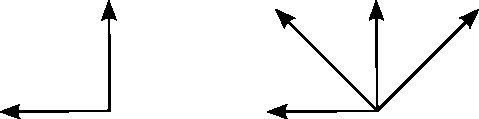
\includegraphics[width=6cm]{masks}
	\caption{Half-mask for the (1)- and (0)-adjacency.\label{fig:masks}}
	\end{center}
\end{figure}

\smallskip
\par In the following, the result of the algorithm will be an image $L$ with one label per connected regions. These labels will be represented by letters. The algorithm is the following
	\begin{itemize}
	\item \textbf{First scan:} We apply one of the two half-masks. For each point $p$:
		\begin{itemize}
		\item If one of its neighbours $q$ has the same gray level, then we propagate the label ($L(p) = L(q)$).
		\item If no neighbour has the same gray level, we create a new label and store it in $L(p)$.
		\item If $p$ has several neighbours with the same gray level but with different labels (labels $a$, $b$), we pick one of them for $p$ (the "lowest" one, for example) and we keep track that both labels correspond to the same region (i.e. $b$ is a synonym of $a$). so called \emph{Collision list}. For example, you could propagate the lowest label in the neighbourhood and make all labels in this neighbourhood "point" to the lowest one.
		\end{itemize}
	\item Figure \ref{fig:connected} illustrates the overall process with four temporary labels and only two remain after the pruning step. As illustrated in this figure, you could implement the collision list as a list where each node has a pointer to its \emph{lowest} parent during the first scan.
	
	\item \textbf{Second scan:} Process the collision list such that each label now points to either to itself or to its root (for example, $D$ is now connected to $A$ instead of $C$). Then, for each pixel we simply remap the labels according to the pruned collision list.
	\end{itemize}

\begin{figure}[ht]
	\begin{center}
	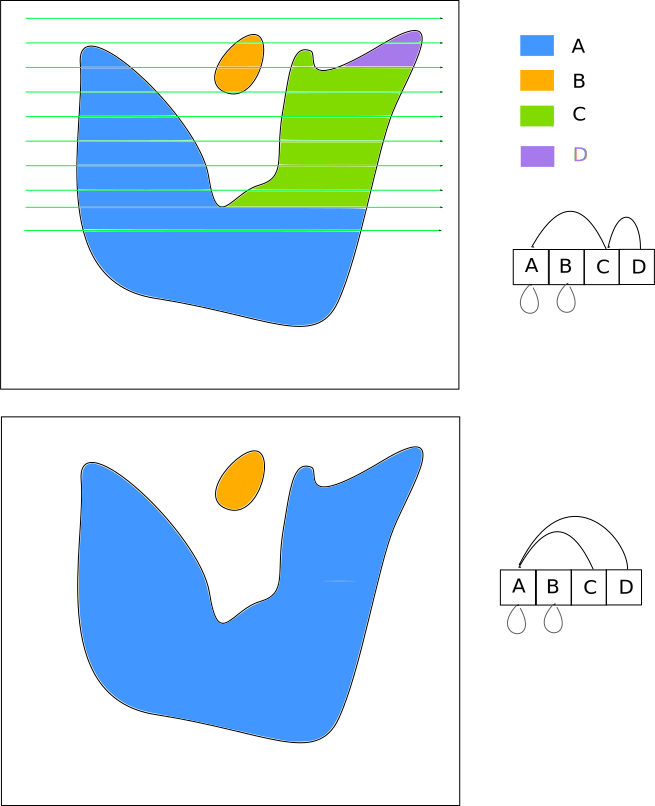
\includegraphics[width=12cm]{connected}
	\caption{Result of the first pass and relabelling.\label{fig:connected}}
	\end{center}
\end{figure}


{\bf Questions:}
\begin{enumerate}
	\item Implement the algorithm described above, for the the $(0)-$ and the $(1)-$adjacencies. Use this algorithm on a grayscale input PGM, then output the label map in PGM format. 
	\item What is the complexity of this algorithm (both memory/time) ?
\end{enumerate}



\section*{Exercise 2 \rm Connected components by Union-find structure}

\par The \emph{Union-find} structure is a very interesting data structure to represent and maintain disjoint sets. Given a set $E$ of elements, such data structure have the following methods: 
\begin{description}
	\item[\texttt{MakeSet(x)}]: creates a set with single element $x\in E$
	\item[\texttt{Find(x)}]: returns the set containing $x$
	\item[\texttt{Union(x,y)}]: compute the union of two disjoint sets.
\end{description}

\par Each disjoint set is represented by one of its elements in $E$. The main interest of this structure is that, for any sequence of size $n$, \texttt{Union} and \texttt{Find} have an amortized complexity of $O(\alpha(n).n)$ (where $\alpha(n)$ is the inverse of the Ackerman function). 

\par The main idea is to represent the collection of sets as a forest of trees (encoded by the \texttt{rank} and \texttt{parent} data members) and to perform \emph{path compression} when doing a \texttt{Find}. Here is the pseudo-code of each function:
\begin{verbatim}
function MakeSet(x)
     x.parent := x
     x.rank   := 0
 
 function Union(x, y)
     xRoot := Find(x)
     yRoot := Find(y)
     if xRoot == yRoot
         return
     if xRoot.rank < yRoot.rank
         xRoot.parent := yRoot
     else if xRoot.rank > yRoot.rank
         yRoot.parent := xRoot
     else
         yRoot.parent := xRoot
         xRoot.rank := xRoot.rank + 1
         
 function Find(x)
     if x.parent != x
        x.parent := Find(x.parent)
     return x.parent
\end{verbatim}

\smallskip
{\bf Questions}
\begin{enumerate}
	\item Implement the union-find structure. You will have to define a C \texttt{struct} (or equivalent) to represent each element of $E$ as a triplet: a rank (\texttt{unsigned int}) a value (which will be the gray value, \texttt{unsigned char} for instance) and a pointer to the parent (element of $E$).
	\item Test the structure on small example.
	\item Implement the connected components extraction algorithm using such structure. For example :  for each pixel, create a set, then for each pixel again, we check the neighbours label and do the union if necessary. Finally, output the final labels using the Find for each pixel.
%% OPTIMISaTION: mélanger avec l'aglo précédent pour ne pas créer de set pour chaque pixel.
	\item What is the computational cost of this algorithm (both memory/time) ?  
	\item Would it be possible to merge the two above mentioned algorithms ? What would be the computational cost ?
\end{enumerate}


\section*{Exercise 3 \rm Comparative evaluation}

\par The idea is to do some experiments to compare the speed of both algorithms.

{\bf Questions:}
\begin{enumerate}
	\item (Image generation) Create two methods parametrized by an image size $n$ and that returns images such that:
	\begin{itemize}
		\item Random image: generate a $n\times n$ image with $m$ ($m<<n$) different gray level for each pixel (randomly selected)
		\item \emph{$n$-fork} image: all even (resp. odd) columns are set to 0 (resp. 1) and the last row contains only 0 pixels. 
	\end{itemize}
	
	\item Test the connected components algorithms on these generated images and compare their efficiency. For example, you could generate several runs with increasing $n$ and output a text file with two columns, $n$ and elapsed time measured using for instance.
	
	\item Conclude on the efficiency of the two previous algorithms.
\end{enumerate}

\smallskip
\par \textbf{Hints:} To measure a delay in C, you can use the library \texttt{<time.h>}, \texttt{<sys/time.h>}\footnote{If you are using gcc, don't forget the "-lrt" option}.
	\begin{itemize}
	\item To declare a timer: \texttt{struct timespec myTimer;}
	\item To measure the current system time: \texttt{clock\_gettime(CLOCK\_REALTIME, \&myTimer);}
	\item To get the informations: \texttt{myTimer} has 2 fields: \texttt{myTimer.tv\_sec} (seconds) and \texttt{myTimer.tv\_nsec} (nanoseconds)
	\end{itemize}
	

\end{document}


